\documentclass[11pt]{article}

\usepackage{graphicx}

% Enable references to labels in the notes
\usepackage{xr-hyper}
\externaldocument{p328_notes}
\usepackage{hyperref}

% Sans fonts
\usepackage{sfmath}
\renewcommand{\familydefault}{\sfdefault}

\newcommand{\COURSE}{PHYS328W}
\newcommand{\LABNUM}{9}
\newcommand{\TITLE}{Operational Amplifiers}
\markright{\COURSE~Lab \LABNUM\ : \TITLE}

\setlength{\textwidth} {6.5 true in}
\setlength{\textheight}{9 true in}
\setlength{\hoffset}   {-0.75 true in}
\setlength{\voffset}   {-0.75 true in}
\setlength{\parindent} {12 pt}
\pagestyle{myheadings}

\begin{document}

\thispagestyle{empty}

\section*{\COURSE\ Lab \LABNUM\ : \TITLE}

This assignment relies on Section~\ref{sec:opamps} of the notes.

\begin{figure}[ht]
  \begin{center}
    \scalebox{0.8}{
      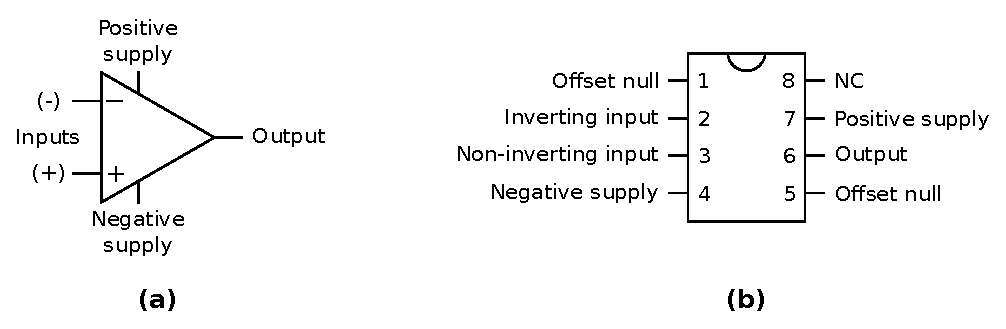
\includegraphics{opamp.eps}
    }
    \caption{(a) Schematic symbol of an operational amplifier, and
      (b) the connection diagram for the 8-pin dual inline package
      (DIP) of the \texttt{LM741} and \texttt{LF411} op amps we will
      use in the lab.}
    \label{fig:opamp}
  \end{center}
\end{figure}

\subsection*{Experiments}


\subsection*{Simulations}


\subsection*{Products}

Upload to Canvas a brief \LaTeX\ report in which you ...
\begin{itemize}
\item 
\end{itemize}

\end{document}
